\documentclass[tikz,border=3pt]{standalone}
\usepackage[utf8]{inputenc}
\usepackage[T1]{fontenc}
\usepackage{lmodern}
\renewcommand{\familydefault}{\sfdefault}
\usepackage{sansmath}\sansmath
\usepackage{chemfig}
\usepackage{pgfplots}\pgfplotsset{compat=1.18,/pgf/number format/use comma,/pgf/number format/1000 sep={.}}
\usetikzlibrary{arrows.meta,calc,positioning,decorations.pathmorphing,patterns}
% paleta del sitio
\definecolor{nar}{HTML}{E8680C}\definecolor{narc}{HTML}{FFB35C}\definecolor{hielo}{HTML}{FFF3E8}
\definecolor{tinta}{HTML}{1D1D1F}\definecolor{gris}{HTML}{6E6E73}\definecolor{lila}{HTML}{7C5CF0}
\definecolor{azul}{HTML}{2F6FD6}\definecolor{menta}{HTML}{17A673}\definecolor{coral}{HTML}{E8342A}
\begin{document}
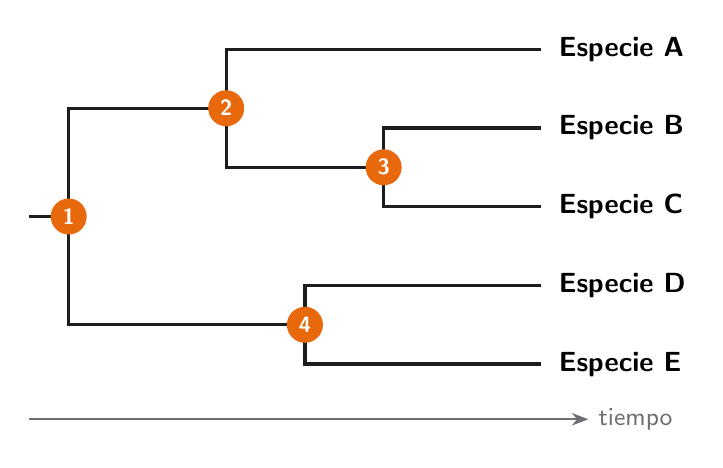
\begin{tikzpicture}[font=\small,rama/.style={tinta,very thick},nodo/.style={circle,fill=nar,text=white,font=\footnotesize\bfseries,inner sep=1.2pt,minimum size=13pt}]
% puntas: A 4, B 3, C 2, D 1, E 0 ; arbol ((A,(B,C)),(D,E))
\draw[rama] (-0.5,1.875) -- (0,1.875);
\draw[rama] (0,1.875) |- (2,3.25);
\draw[rama] (0,1.875) |- (3,0.5);
\draw[rama] (2,3.25) |- (6,4);
\draw[rama] (2,3.25) |- (4,2.5);
\draw[rama] (4,2.5) |- (6,3);
\draw[rama] (4,2.5) |- (6,2);
\draw[rama] (3,0.5) |- (6,1);
\draw[rama] (3,0.5) |- (6,0);
\node[nodo] at (0,1.875) {1};
\node[nodo] at (2,3.25) {2};
\node[nodo] at (4,2.5) {3};
\node[nodo] at (3,0.5) {4};
\foreach \n/\y in {A/4,B/3,C/2,D/1,E/0} \node[anchor=west,font=\bfseries] at (6.1,\y) {Especie \n};
\draw[-{Stealth[length=6pt]},gris,thick] (-0.5,-0.7) -- (6.6,-0.7) node[anchor=west,text=gris] {tiempo};
\end{tikzpicture}
\end{document}
